\section{Real Clock}\label{sc:realClock}

Short introduction to real clocks here.
An attempt to synchronize discrete systems around real time, with different algorithms making different balances between precision and resource requirements.

PTP (most important)
NTP
RBIS
The real clocks are integrated circuit in electronics with the alternate power source for counting time when the electronics is off, which are used in the systems that needs to keep accurate time. Most of the systems uses crystal oscillator. Because of the clock drift there is a need to synchronize clocks. The two most used algorithms for it is PTP(Precision Time Protocol) and NTP(Network time Protocol) will be described separately below.

\subsection{The need for real clocks}

Why do we need real clocks? Can't we just use the logical ones u just talked about?
Some system needs to know real time(e.g. stock market, bank systems). Logical clocks wont work in this case, because we need precise time of transactions.
Some system needs to know real time(e.g. stock market, bank systems). Logical clocks wont work in this
case, because we need precise time of transactions.


\subsection{PTP - Precision Time Protocol}

- IEEE 1588
- Explain the basics. Applications?
- Why is suited/designed for packet-switched networks?
- Does it scale well? Performance?
- Show Phase 1 and Phase 2.
- Master slave.

\subsection{Software vs. hardware}
\subsection{NTP - Network time Protocol}

Why is it good to timestamp at the lowest layer possible in the network stack close to transmitting via the physical layer?
NTP was design by David L. Mills and it is operational since before 1985. It is one of the oldest protocol in
current use. The core principal of the protocol is server-client communication. In the stratum 0 is located
most accurate timekeepers (e.g. GPS, radio clock, etc.). These timekeepers are directly interfacing to the
stratum 1 servers, also between same level stratum severs can be interface to each other as shown in \ref{fig:NTP}.

\begin{figure}[h!]\label{}
	\centering
	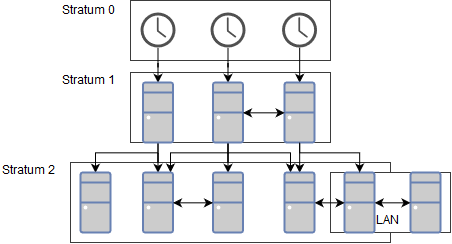
\includegraphics[scale=0.4]{synchronization/fig/NTP.png}
	\caption{An DFA that accepts any input that contains two '1' symbols in a row}
	\label{fig:NTP}
\end{figure}
Pros of network time protocol is that the client can be connected to more then one severer to get time, itis cheaper to develop NTP then PTP. Has feature called "Insane Time" which prevents synchronization witha server who is 1024 seconds apart.


Cons requires at lest one interface through wide area network which leads to security issues. Below stratum
15 devices are held unsynchronized.